\section{Messstruktur für Analog-Digital-Wandler}
	
	Nach der Einführung in die grundlegenden Funktionen von LabView sollte an dem zweiten Tag eine Messstruktur programmiert werden.
	Dazu wurde den Studenten jeweils ein Funktionsgenerator und ein Analog-Digital-Wandler zur Verfügung gestellt.
	Über diesen Wandler ließ sich der Funktionsgenerator an den Computer schließen.
	Da es sich hierbei um einen ADC von NationalInstruments handelte, erkannte LabView diesen sofort.
	
	\subsection{DAQ-Assistant}
	
		Mit dem vorprogrammierten Express-VI, dem DAQ-Assistant (siehe Abb. \ref{fig:daq}), konnte gemessen werden.
		\begin{figure}[ht]
			\centering
			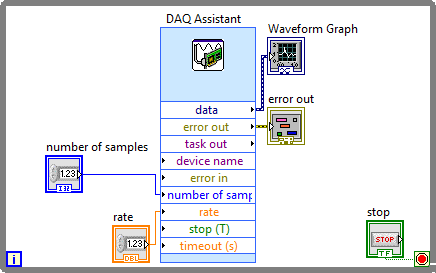
\includegraphics[width=\textwidth]{pic/daq.png}
			\caption{Diese Abbildung stellt das Express-VI "DAQ-Assistant" dar. Darauf sind die verschiedenen Ein- und Ausgänge zu sehen.}
			\label{fig:daq}	
		\end{figure}
		Lediglich die Anzahl der Datenpunkte und die Messrate mussten dem DAQ-Assistant geliefert werden damit ein Waveform-Graph aus dem Array, welches der "data"-Ausgang ausgab, das Bild in Abb. \ref{fig:daq_sig} erzeugt werden konnte. 
		\begin{figure}[h]
			\centering
			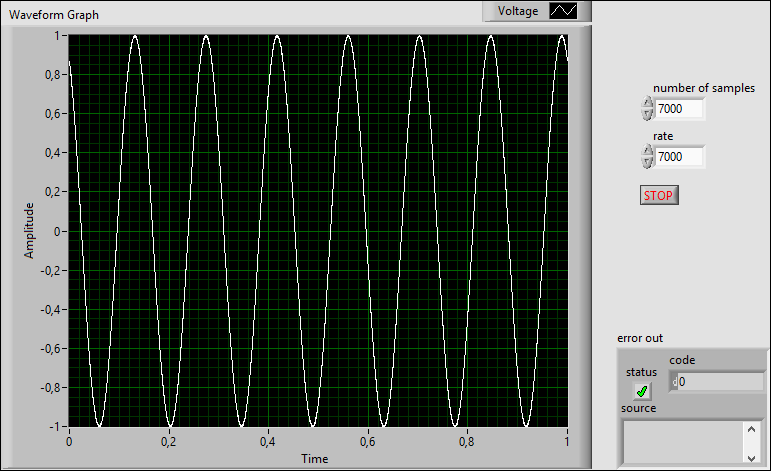
\includegraphics[width=\textwidth]{pic/daq_sig.png}
			\caption{Diese Abbildung stellt das Frontpanel eines VIs mit dem DAQ-Assistant und Controls für Messrate und Anzahl der Datenpunkte dar.}
			\label{fig:daq_sig}	
		\end{figure}
		Das aufgezeichnete Signal stimmte mit dem überein, was an dem Funktionsgenerator eingestellt wurde.
	
	\newpage
	\subsection{Programmieren einer eigenen Messstruktur}
	
		Da lediglich eine Anzeige des gemessenen Signals oft nicht reicht, musste eine Messstruktur programmiert werden, die den Umfang des DAQ-Assistants übersteigt und weiter manuell angepasst werden kann.
		
		Aufgrund von Problemen bei Wartungsarbeiten ließen sich die Computer jedoch gegen Mittag nicht mehr bedienen, weswegen das Fertigstellen des Programms auf den dritten Tag verschoben wurde. 
	